- explain procedure:
1. find most suitable $m$ for all machine learning techniques via cross-validation and find best hyperparameters for best $m$ (if applicable) via cross-validation
2. compute test accuracy, compute confusion matrix, ROC plot

\subsection{Majority Predictor}
- CV accuracy and test accuracy constant for all $m$ (in general, different)
- take majority predictor as a reference for the performance of the other prediction algorithms

\begin{figure}
  \centering
  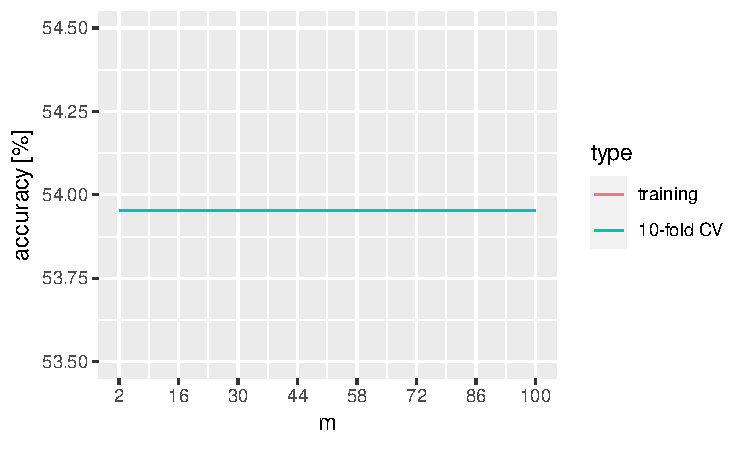
\includegraphics[width=\textwidth]{major_acc_vs_m.pdf}
  \caption{accuracy}
\end{figure}

- test accuracy: \SI{55.54}{\percent}



\begin{table}
\centering
\begin{tabular}{c|c|c|c|c}
  \backslashbox{predicted}{true} & $0$ & $1$ \\
 \hline
 $0$ & $0$ & $0$ \\  
 \hline
 $1$ & $309$ & $386$    
\end{tabular}
 \caption{confusion matrix of majority predictor on test set}
\end{table}

\subsection{Logistic Regression}
- test accuracy: \SI{56.70}{\percent} at $m=4$
- training accuracy becomes much larger because model stores training examples , CV accuracy remains roughly constant (decreases slightly)

\begin{figure}
  \centering
  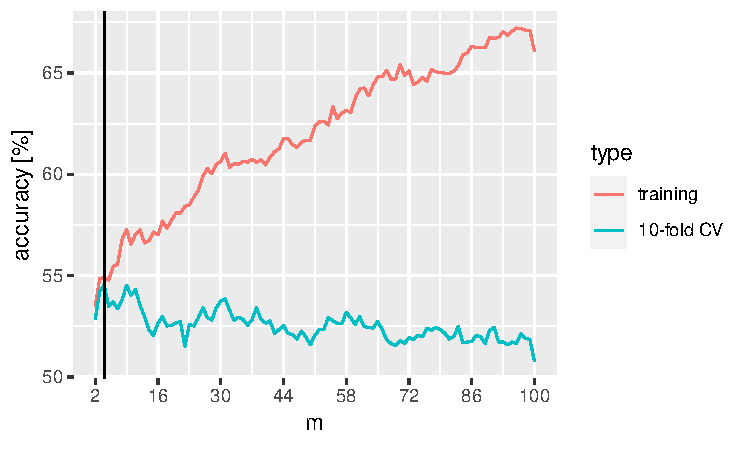
\includegraphics[width=\textwidth]{log_acc_vs_m.pdf}
  \caption{accuracy}
\end{figure}

- model distinguishes, better than majority predictor as also Bitcoin down is predicted

\begin{figure}
  \centering
  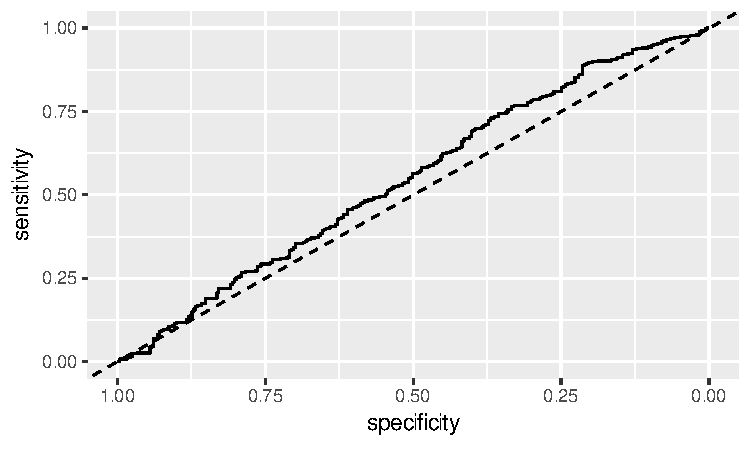
\includegraphics[width=\textwidth]{log_roc.pdf}
  \caption{roc curve for logistic predictor}
\end{figure}

\begin{table}
\centering
\begin{tabular}{c|c|c}
  \backslashbox{predicted}{true} & $0$ & $1$ \\
 \hline
 $0$ & $77$ & $73$ \\  
 \hline
 $1$ & $232$ & $313$    
\end{tabular}
 \caption{confusion matrix of logistic regression predictor on test set}
\end{table}

\begin{table}
\centering
\begin{tabular}{c||c|c|c|c}
coefficient & estimate & std. & $z$ score & $P(>|z|)\,[\%]$ \\
 \hline
 \hline
(intercept) & $-0.15$ & $0.22$ & $-0.688$ & $49.13$ \\  
 \hline
 market price ($t_{-2}$) & $0.45$ & $-0.60$ & $0.764$ & $44.51$\\   
 \hline
market price ($t_{-1}$) & $0.71$ & $0.82$ & $0.874$ & $38.20$\\
\hline
market price ($t_{0}$) & $-0.65$ & $0.57$ & $-1.121$ & $26.22$\\
\hline
\# transactions ($t_{-2}$) & $-0.28$ & $0.27$ & $-1.040$ & $29.81$\\
\hline
\# transactions ($t_{-1}$) & $0.20$ & $0.32$ & $0.624$ & $53.28$\\
\hline
\# transactions ($t_{0}$) & $0.11$ & $0.27$ & $0.394$ & $69.32$\\
\hline
avg. block size ($t_{-2}$) & $-0.10$ & $0.28$ & $-0.252$ & $80.10$\\
\hline
avg. block size ($t_{-1}$) & $-0.54$ & $0.32$ & $-1.682$ & $9.25$\\
\hline
avg. block size ($t_{0}$) & $0.69$ & $0.28$ & $2.501$ & $1.24$\\
\hline
hash rate ($t_{-2}$) & $-0.10$ & $0.26$ & $-0.171$ & $86.44$\\
\hline
hash rate ($t_{-1}$) & $-0.10$ & $0.28$ & $-0.043$ & $96.56$\\
\hline
hash rate ($t_{0}$) & $-0.10$ & $0.26$ & $-0.029$ & $97.67$\\
\end{tabular}
 \caption{confusion matrix of logistic regression predictor on test set}
\end{table}

\begin{table}
\centering
\begin{tabular}{c|c}
coefficient & $\sqrt{VIF}$ \\
 \hline
 \hline
 market price ($t_{-2}$) & $4.69$ \\   
 \hline
market price ($t_{-1}$) & $6.64$ \\
\hline
market price ($t_{0}$) & $4.82$ \\
\hline
\# transactions ($t_{-2}$) & $1.68$ \\
\hline
\# transactions ($t_{-1}$) & $2.01$ \\
\hline
\# transactions ($t_{0}$) & $1.70$ \\
\hline
avg. block size ($t_{-2}$) & $1.78$ \\
\hline
avg. block size ($t_{-1}$) & $2.08$ \\
\hline
avg. block size ($t_{0}$) & $1.79$\\
\hline
hash rate ($t_{-2}$) & $1.45$ \\
\hline
hash rate ($t_{-1}$) & $1.55$ \\
\hline
hash rate ($t_{0}$) & $1.46$ \\
\end{tabular}
 \caption{sqrt(VIF) for logistic regression}
\end{table}

\section{K-Nearest Neighbors Algorithm}
- test accuracy: \SI{51.80}{\percent} at $m=91$

\begin{figure}
  \centering
  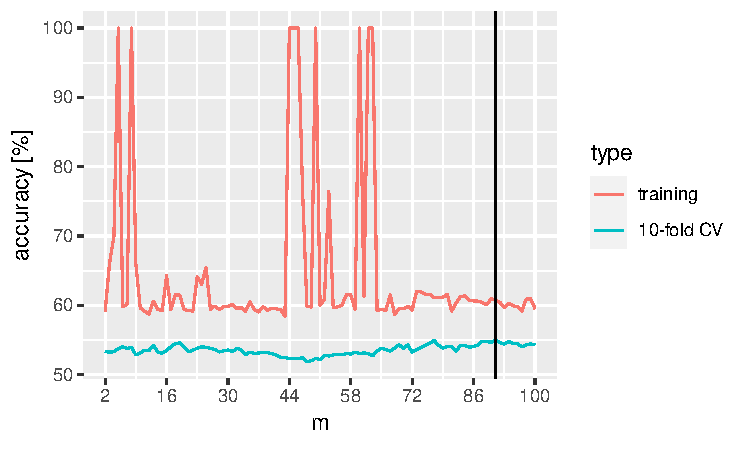
\includegraphics[width=\textwidth]{knn_acc_vs_m.pdf}
  \caption{accuracy knn}
\end{figure}

\begin{figure}
  \centering
  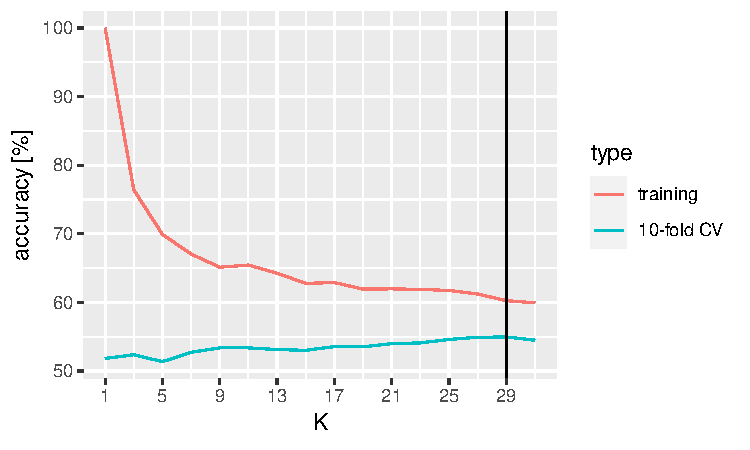
\includegraphics[width=\textwidth]{knn_acc_vs_K.pdf}
  \caption{accuracy knn vs. K}
\end{figure}

\begin{figure}
  \centering
  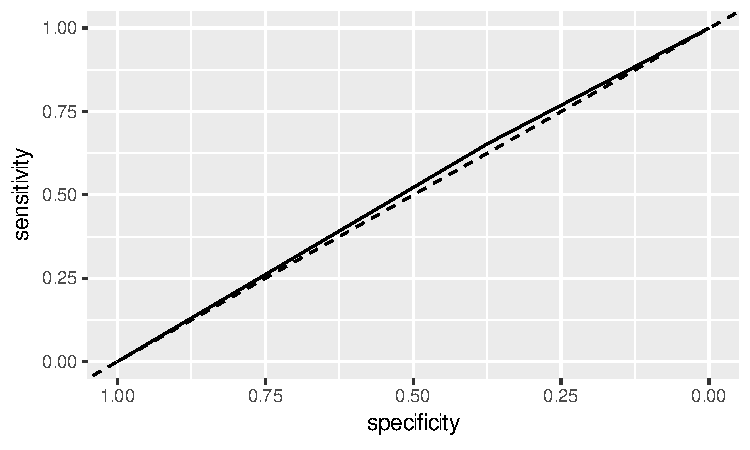
\includegraphics[width=\textwidth]{knn_roc.pdf}
  \caption{knn ROC}
\end{figure}

\begin{figure}
  \centering
  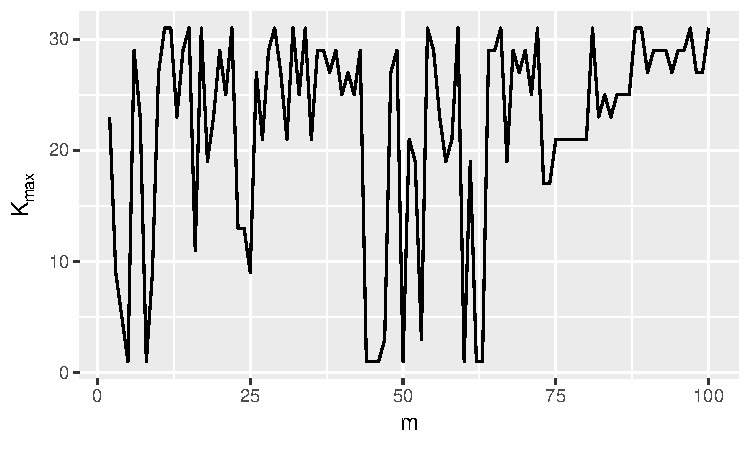
\includegraphics[width=\textwidth]{knn_K_max.pdf}
  \caption{knn K max}
\end{figure}

\begin{table}
\centering
\begin{tabular}{c|c|c}
  \backslashbox{predicted}{true} & $0$ & $1$ \\
 \hline
 $0$ & $115$ & $133$ \\  
 \hline
 $1$ & $194$ & $253$    
\end{tabular}
 \caption{confusion matrix of knn on test set}
\end{table}

\section{Deep Neural Network}

